\section{绪论}

\subsection*{选题背景}

\begin{frame}
	\frametitle{分布式计算框架}
	\vspace{-1.2em}
	\begin{columns}[t]
		\column{0.48\textwidth}
		\begin{block}{早期计算框架\\(Hadoop, Spark, Horovod)}
			\begin{itemize}
				\item 单一的任务类型
				\item 固定的并行模式
				\item 有限的表达能力
			\end{itemize}
		\end{block}
		\column{0.48\textwidth}
		\begin{block}{计算任务的变化}
			\begin{itemize}
				\item 异构任务
				\item 复杂的组织结构
				\item 实时计算、在线处理
			\end{itemize}
		\end{block}
	\end{columns}
	\begin{columns}[onlytextwidth]
		\column{0.33\textwidth}	
		\begin{figure}
			\centering
			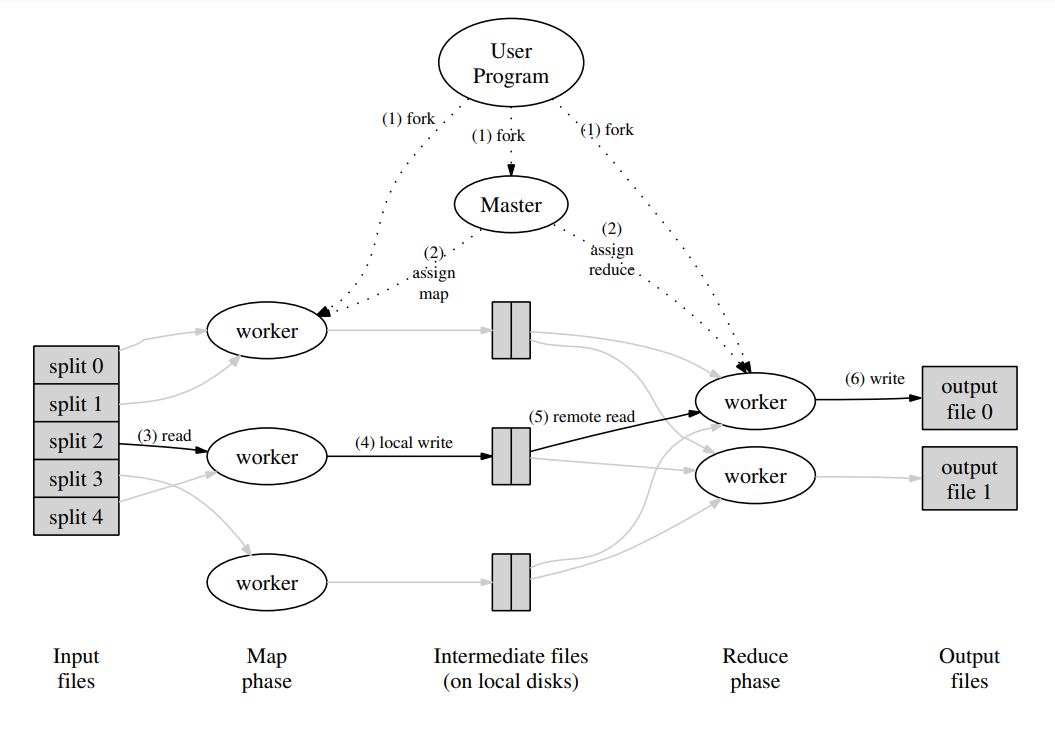
\includegraphics[width=\textwidth]{image/chap01/mapreduce.png}	
			\caption{Mapreduce}
		\end{figure}
		\column{0.33\textwidth}	
		\begin{figure}
			\centering
			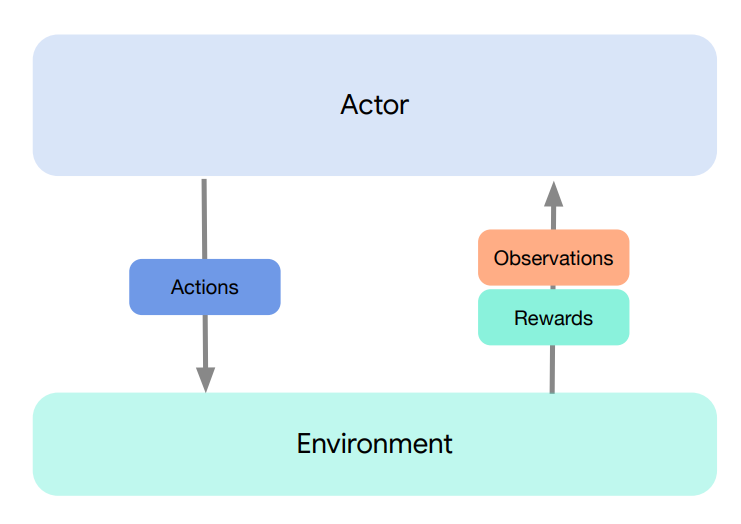
\includegraphics[width=\textwidth]{image/chap01/acme.png}	
			\caption{强化学习}
		\end{figure}
		\column{0.33\textwidth}	
		\begin{figure}
			\centering
			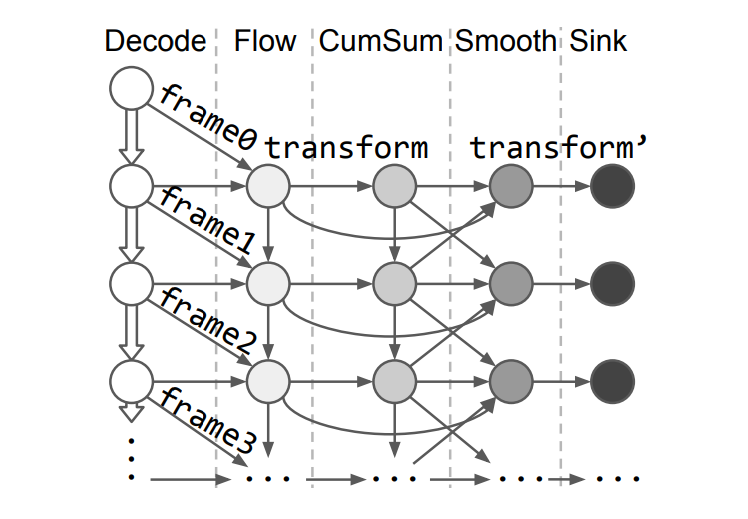
\includegraphics[width=\textwidth]{image/chap01/ray.png}
			\caption{视频流处理}
		\end{figure}
	\end{columns}
\end{frame}

\frame{
	\frametitle{新型计算框架Ray}
	\begin{columns}[onlytextwidth]
		\column{0.31\textwidth}
		\vspace{-0.5em}
		\begin{block}{通用\&实时}
			\begin{itemize}
				\item 细粒度任务调度 \\ 函数为单位
				\item \textbf{集群内存管理} \\ 数据随调度移动
			\end{itemize}
		\end{block}
		\begin{block}{集群内存管理}
			\begin{itemize}
				\item 依赖解析机制
				\item 分布式内存存储Plasma
			\end{itemize}
		\end{block}
		\column{0.68\textwidth}
		\vspace{-0.5em}
		\begin{figure}
			\centering
			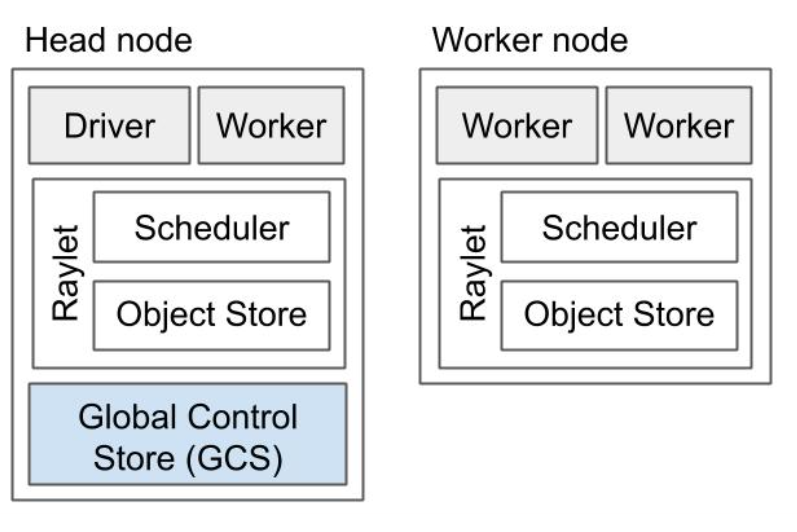
\includegraphics[width=0.95\textwidth]{image/chap02/ray_arch.png}
			\caption{Ray集群架构}
		\end{figure}
	\end{columns}
}

\begin{frame}
	\frametitle{硬件的变化}

	\vspace{-1.5em}
	\begin{columns}[t]
		\column{0.47\textwidth}
		\begin{block}{分布式内存存储Plasma}
			\begin{itemize}
				\item 内存对象的网络传输
				\item 大小不一的对象
				\item \textbf{是否充分利用网络?}
			\end{itemize}
		\end{block}
		\column{0.47\textwidth}
		\begin{block}{Infiniband高速网络}
			\begin{itemize}
				\item 低延迟:$\thicksim 1\mu s$
				\item 高带宽:200Gb/s
				\item 链路层容错
				\item \textbf{RDMA}
			\end{itemize}
		\end{block}
	\end{columns}

	\begin{columns}[onlytextwidth]
		\column{0.3\textwidth}
		\begin{figure}
			\centering
			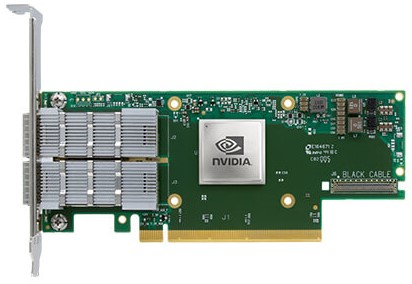
\includegraphics[scale=0.3]{image/presentation/hca.jpg}
			\caption{HDR IB网卡}
		\end{figure}
	
		\column{0.7\textwidth}
		\begin{figure}
			\centering
			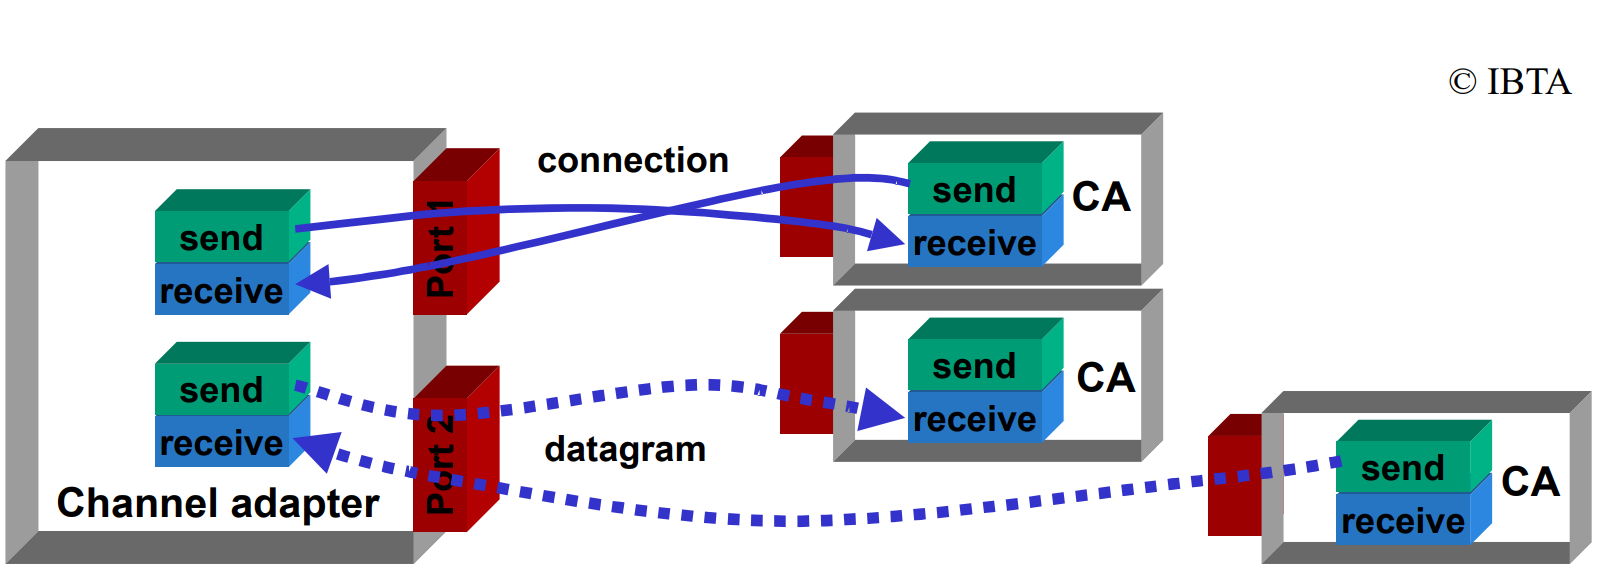
\includegraphics[scale=0.13]{image/chap01/qp.png}
			\caption{IB传输层模型}
		\end{figure}
	\end{columns}
		
\end{frame}

\begin{frame}
	\frametitle{远程直接内存访问(Remote Direct Memory Access,RDMA)}
	\begin{columns}[onlytextwidth]
		\column{0.25\textwidth}
		\begin{block}{\textbf{用户态}网络栈}
			\begin{itemize}
				\item 内核旁路
				\item 零拷贝
				\item CPU卸载
			\end{itemize}
		\end{block}
		\column{0.73\textwidth}
		\vspace{1.5em}
		\begin{figure}
			\centering
			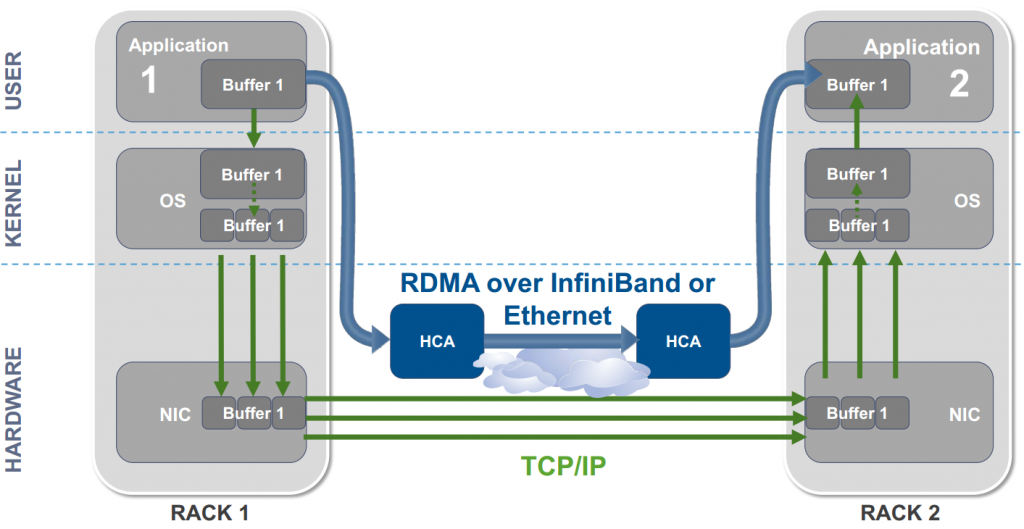
\includegraphics[width=\textwidth]{image/presentation/rdma.png}
			\caption{RDMA示意图}
			\label{fig:rdma}
		\end{figure}
	\end{columns}
\end{frame}

\subsection*{国内外研究现状}
\begin{frame}
	\frametitle{基于RDMA的内存系统}

	

\end{frame}

\subsection*{本文的工作}
\begin{frame}
	\begin{block}{如何为Plasma提供原生RDMA支持?}
		我们的实现兼容~以太网~和~Infiniband
	\end{block}
	\begin{block}{大小不一的内存对象,如何性能最佳?}
		基于对象大小的混合传输协议
	\end{block}
	\begin{block}{如何测试传输性能?}
		基于MPI的多节点测试;确定了最优决策参数
	\end{block}
\end{frame}
